\begin{figure}
  \centering
    \includegraphics[width=0.75\textwidth]{Figures/p_vs_K_fm.pdf}
  \caption{Reproduction of Figure 12b of Flache and Macy (2011). The average
    polarization decreases with $K$. However, as shown in subsequent figures,
    this does not mean trials with high polarization never obtain.
  }
  \label{fig:p_vs_K_fm}
\end{figure}


\begin{figure}[h!]
  \centering
    \begin{subfigure}[t]{\textwidth}
      \centering
      \includegraphics[width=.65\textwidth]{Figures/connected-caveman-over-K.pdf}
      \caption{Final polarizations for the non-random connected caveman graph.}
      \label{fig:connected-caveman-trials}
    \end{subfigure}
    \begin{subfigure}[t]{\textwidth}
      \centering
      \includegraphics[width=.65\textwidth]{Figures/random-shortrange-over-K.pdf}
      \caption{Final polarizations for the non-random connected caveman graph.}
      \label{fig:random-shortrange-trials}
    \end{subfigure}
    \begin{subfigure}[t]{\textwidth}
      \centering
      \includegraphics[width=.65\textwidth]{Figures/random-anyrange-over-K.pdf}
      \caption{}
      \label{fig:random-anyrange-trials}
    \end{subfigure}
  \caption{Even in the non-random connected caveman structure, there is 
    variation in the final polarization for different values of $K$. Highly
    polarized final states may obtain. 100 trials are shown and comprise the
    average. The circle shows the result for one trial of the configuration
    reused to make Figure~\ref{fig:single-ic-histogram}.
  }
  \label{fig:single-experiments-over-k}
\end{figure}


\begin{figure}[h!]
  \centering
    \includegraphics[width=.75\textwidth]{Figures/final-initial-pol-regplot.pdf}
  \caption{Final and initial polarizations shown for $K=2$ with the connected 
    caveman network. Final polarizations are same as in the $K=2$ column of 
    Figure~\ref{fig:connected-caveman-trials}}
  \label{fig:final-initial-pol-regplot}
\end{figure}

\begin{figure}[h!]
  \centering
    \includegraphics[width=.75\textwidth]{Figures/caveman-highpol-histogram-10k-its.pdf}
  \caption{Distribution of final polarizations at iteration 10000
  starting from initial conditions
  of the connected caveman trial with the largest final polarization with $K=2$.
  The distribution is skewed towards final polarizations considerably larger
  than the mean polarization of 0.41 for the connected caveman experiment
  with $K=2$. 
  }
  \label{fig:highpol-histogram}
\end{figure}

% \begin{figure}[t!]
%   \centering
%   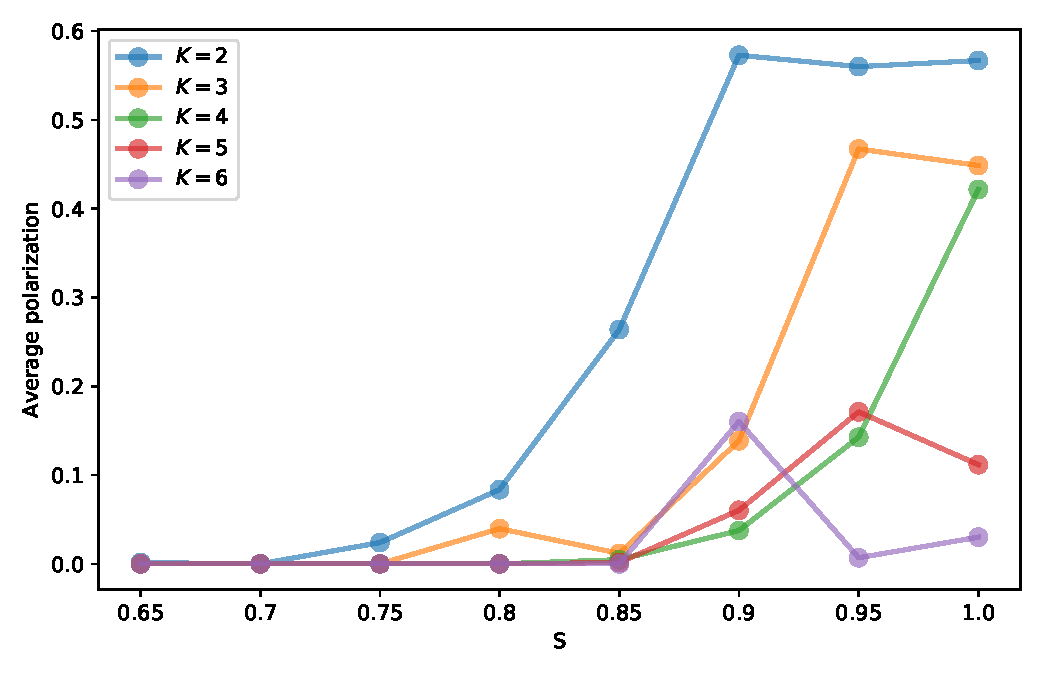
\includegraphics[width=0.75\textwidth]{Figures/P_vs_S_for_K.pdf}
%   \caption{
%     Average final polarization becomes non-zero then increases as
%     the width of the uniform distribution of initial opinions increases.
%     The width must be larger and larger as the cultural complexity $K$ 
%     increases for the system to achieve non-zero final polarization. This
%     condition is identical to the bottom row of each heatmap in 
%     Figure \ref{fig:heatmaps}. Each
%     data point is the average of fifty trials. Each trial ran over 
%     10k timesteps. 
%   }
%   \label{fig:p_vs_s_for_k}
% \end{figure}


\begin{figure}[t!]
  \centering
    \includegraphics[width=0.75\textwidth]{Figures/s_k_zoom_2-6_mean.pdf}
  \caption{Zoom-in on \emph{average} polarization versus $S$ for $K=6$. 
  Different experiment run from Figure~\ref{fig:p_vs_s_for_k}. 
  Same data as in Figure~\ref{fig:zoom_median}.
  Average taken over 100 trials.}
  \label{fig:zoom_average}
\end{figure}

\begin{figure}[h!]
  \centering
    \includegraphics[width=0.75\textwidth]{Figures/s_k_zoom_2-6_median.pdf}
  \caption{Zoom-in on \emph{median} polarization versus $S$ for $K=2,3,4,5,6$. 
    Median polarization for $K=5$ and $K=6$ are both flat at zero; $K=5$ 
    data is obscured by $K=6$.
    Different experiment run from Figure~\ref{fig:p_vs_s_for_k}.
    Same data as in Figure~\ref{fig:zoom_average}.
    Median taken over 100 trials.
  }
  \label{fig:zoom_median}
\end{figure}


\begin{figure}[h!]
  \centering
  \begin{subfigure}[t]{\textwidth}
    \centering
    \includegraphics[width=0.5\textwidth]{Figures/single_S_K=2.pdf}
  \end{subfigure} \\
  \begin{subfigure}[t]{0.49\textwidth}
      \centering
      \includegraphics[width=\textwidth]{Figures/single_S_K=3.pdf}
      % \caption{}
  \end{subfigure}
  ~
  \begin{subfigure}[t]{0.49\textwidth}
      \centering
      \includegraphics[width=\textwidth]{Figures/single_S_K=4.pdf}
      % \caption{}
  \end{subfigure} \\
  \begin{subfigure}[t]{0.49\textwidth}
      \centering
      \includegraphics[width=\textwidth]{Figures/single_S_K=5.pdf}
      % \caption{}
  \end{subfigure}
  ~
  \begin{subfigure}[t]{0.49\textwidth}
      \centering
      \includegraphics[width=\textwidth]{Figures/single_S_K=6.pdf}
      % \caption{}
  \end{subfigure}
  \caption{The average polarization is actually very noisy because 
    final polarizations find a large range of values. Even for $K=6$, there
    are a significant number of trials that end in a non-zero polarization
    state. We need to figure out what causes this. Network configuration?
    Initial conditions? We need to do two tests: hold one or the other 
    constant and vary the other.
  }
  \label{fig:single_S_K}
\end{figure}


\begin{figure}[t!]
  \centering
      \begin{subfigure}[t]{0.49\textwidth}
          \centering
          \includegraphics[width=\textwidth]{Figures/noisecomm_K=2.pdf}
          \caption{}
      \end{subfigure}
      ~
      \begin{subfigure}[t]{0.49\textwidth}
          \centering
          \includegraphics[width=\textwidth]{Figures/noisecomm_K=3.pdf}
          \caption{}
      \end{subfigure} \\
      \begin{subfigure}[t]{0.49\textwidth}
          \centering
          \includegraphics[width=\textwidth]{Figures/noisecomm_K=4.pdf}
          \caption{}
      \end{subfigure}
      ~
      \begin{subfigure}[t]{0.49\textwidth}
          \centering
          \includegraphics[width=\textwidth]{Figures/noisecomm_K=5.pdf}
          % 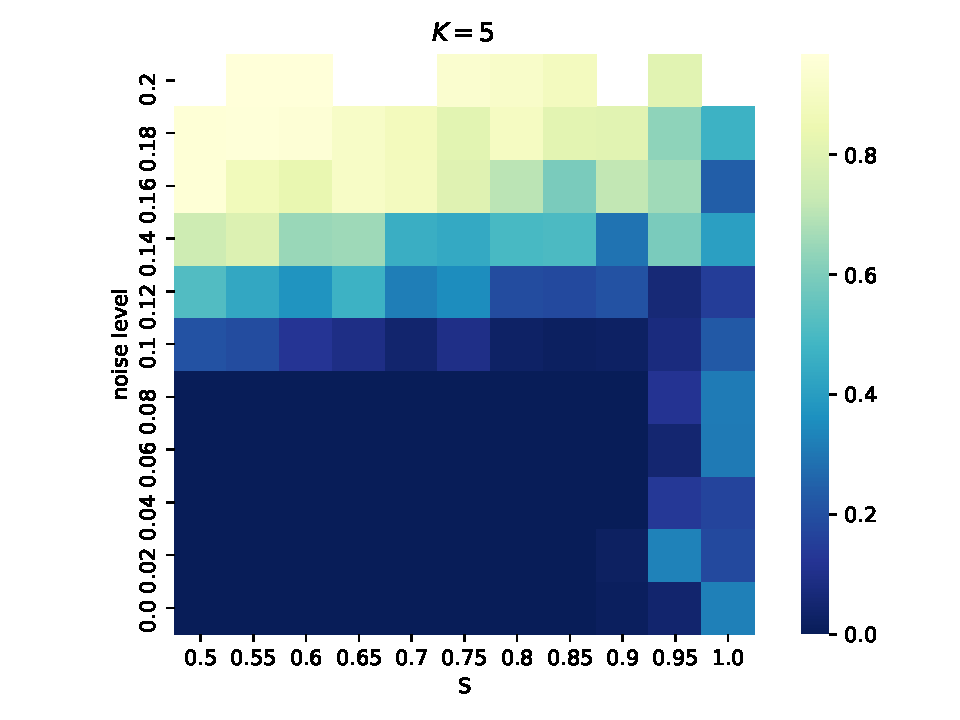
\includegraphics[width=\textwidth]{Figures/p_v_noise_k=5.pdf}
          \caption{}
      \end{subfigure} \\
  \caption{Final average polarization varies with both the width of the
    uniform distribution of initial opinion magnitudes and the noise level in
    the opinion updates. Noisy opinion updates can perturb the system away from
    situations where homogeneity of opinion would otherwise obtain. $K=2,3,4,5$
    are shown. The value in each square of the heatmap is the average of
    fifty trials. Each trial ran over 10k timesteps.
  }
  \label{fig:heatmaps}
\end{figure}


\begin{figure}[t!]
  \centering
      \begin{subfigure}[t]{0.49\textwidth}
          \centering
          \includegraphics[width=\textwidth]{Figures/noisecomm_S=0p5_K=2.pdf}
          \caption{}
      \end{subfigure}
      ~
      \begin{subfigure}[t]{0.49\textwidth}
          \centering
          \includegraphics[width=\textwidth]{Figures/noisecomm_level=0p10_K=2.pdf}
          \caption{}
      \end{subfigure} \\
      \begin{subfigure}[t]{0.49\textwidth}
          \centering
          \includegraphics[width=\textwidth]{Figures/noisecomm_S=0p5_K=4.pdf}
          \caption{}
      \end{subfigure}
      ~
      \begin{subfigure}[t]{0.49\textwidth}
          \centering
          \includegraphics[width=\textwidth]{Figures/noisecomm_level=0p10_K=4.pdf}
          \caption{}
      \end{subfigure} \\
      \begin{subfigure}[t]{0.49\textwidth}
          \centering
          \includegraphics[width=\textwidth]{Figures/noisecomm_S=0p5_K=6.pdf}
          \caption{}
      \end{subfigure}
      ~
      \begin{subfigure}[t]{0.49\textwidth}
          \centering
          \includegraphics[width=\textwidth]{Figures/noisecomm_level=0p10_K=6.pdf}
          \caption{}
      \end{subfigure}
  \caption{Details of final polarizations and average for a fixed 
    maximum initial opinion magnitude and level of noise communication for many
    values of cultural complexity, $K$
  }
  \label{fig:single-runs-commnoise}
\end{figure}

% % Figures/noisecomm_S=0.5_K=3.pdf
% Figures/noisecomm_S=0.5_K=4.pdf
% % Figures/noisecomm_S=0.5_K=5.pdf
% Figures/noisecomm_S=0.5_K=6.pdf

% % Figures/noisecomm_level=0.10_K=3.pdf
% Figures/noisecomm_level=0.10_K=4.pdf
% % Figures/noisecomm_level=0.10_K=5.pdf
% Figures/noisecomm_level=0.10_K=6.pdf
